\section{Data}

\subsection{The Market and Demand}

The middle European electricity market cannot be restricted to one country only. However, we focus on Germany as the four biggest Players (EoN, RWE, Vattenfal and EnBW) and the most important electricity exchange in the Region, the EEX are situated there. There are, however, significant import capacities from the neighboring countries (see \cite{Ellersdorfer2005}p. 30). Other electricity Exchanges are the EXAA in Austria, the APX in The Netherlands and the Powernext in France. Apart from energy exchanges, there are OTC Markets as well for which data are hard to get. However, prices at the electricity exchanges are generally regarded as a reliable price signal for the OTC Market. \cite{Holler2006} compare OTC prices and prices from the exchanges (EEX and EXAA) in Austria and Germany and conclude that both prices seem to reflect one market in the respective countries. Furthermore, they look at correlations between market prices at the different exchanges and come to the conclusion, that prices at the EEX, EXAA and Powernext are highly correlated. However, only about four percent of the French electricity consumption is traded at the spot market and the whole French industry is heavily dominated by EDF which casts some doubt on whether there is a working electricity market in France. This is why we do not model France as a strategic part of the market which does not mean that research on that topic would not be interesting. Furthermore, the only countries where transmission lines are not congested at the moment, are Germany and Austria\footnote{An Overview of Current Cross-boarder Congestion Management Methods in Europe, www.etso-net.org} which is why we restrict our analysis to the two latter countries.
\begin{figure}[h]
\centering
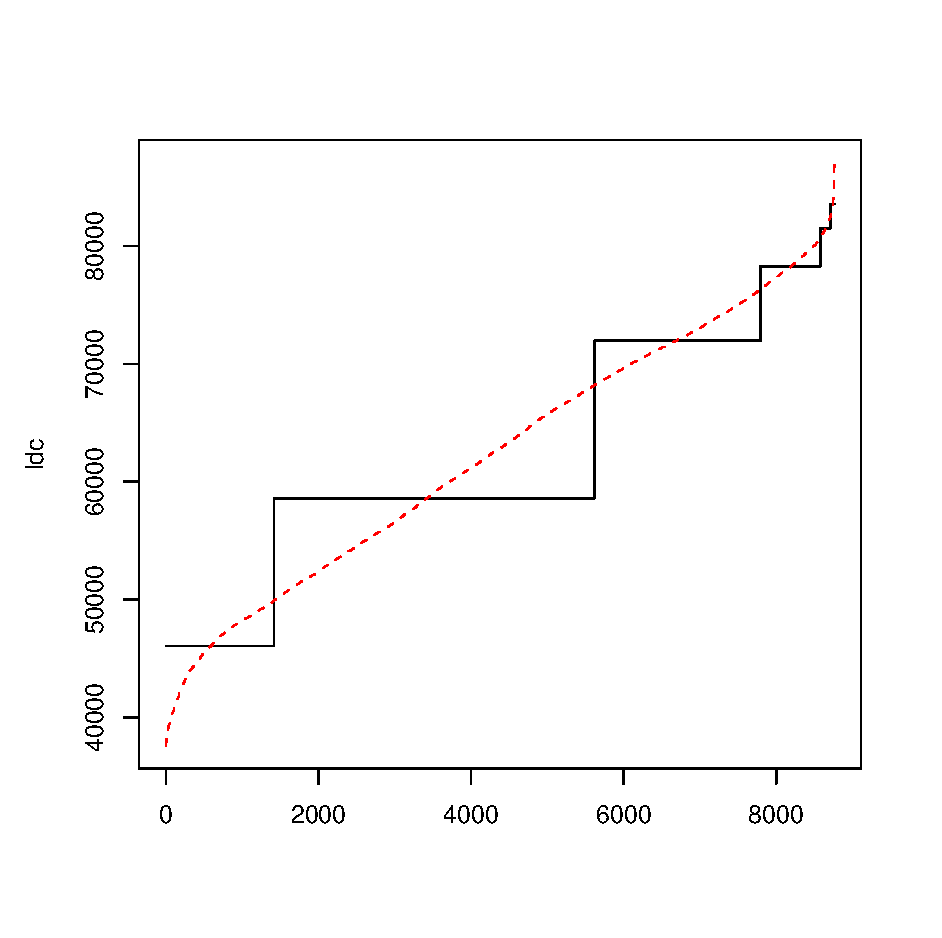
\includegraphics[width=.5\textwidth]{data/ldc}
      \label{fig:ldc}
      \caption{Load Duration Curve in MWh for Austria and Germany}
      source: UCTE\footnote{http://www.ucte.org/}
\end{figure}
Figure \ref{fig:ldc} shows the load duration curve for Germany and Austria. It can be seen that there are a few extreme demand spikes and normal values between roughly 80.000 and 40.000 MWh.. To get a picture of the states of the market, Prices from the EEX were plotted against total electricity load in the economy. The correlation is evident. Furthermore, there seems to be an upper bound to capacity which leads prices to explode if that bound is approached. Of course, quantity is not the only factor to explain prices and so there is uncertainty associated with our model. It could well be that demand in the neighboring countries is lower than expected during a high demand period in Germany and so this free capacities dampen the price spike at the EEX. All these uncertain other developments shall be accounted for by our measure of uncertainty in our model. Please note that if we plot prices and quantities at the EEX there seems to be no correlation at all. This is another sign that the exchange just does not cover the whole market and that there is a closely related OTC market which, together with the exchange forms the actual market for electricity.
\begin{figure}[h]
\centering
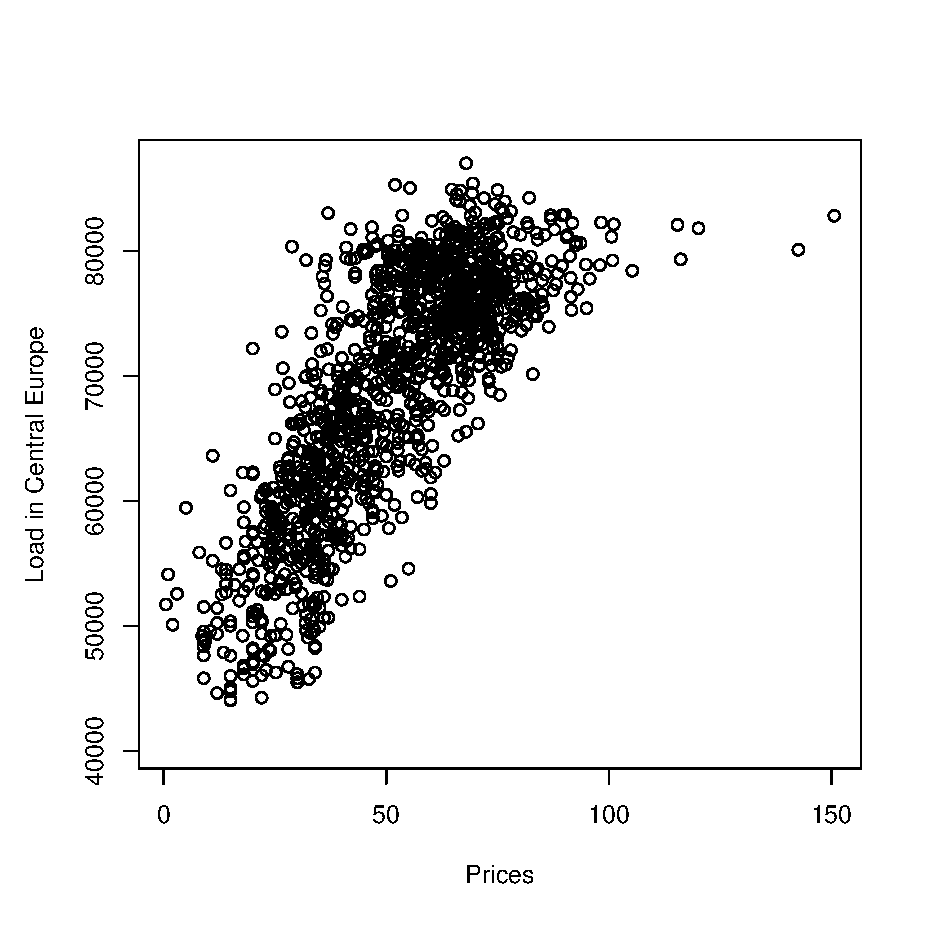
\includegraphics[width=.5\textwidth]{data/korrelation}
      \label{fig:ldc}
      \caption{Load Duration Curve in MWh for Austria and Germany}
      source: UCTE and EEX \footnote{http://www.ucte.org/; http://www.eex.com/}
\end{figure}
To account for different states of the market, demand functions for cases where prices were bigger than 100, between 80 and 100 and so on were constructed. \cite{Neuhoff2005} use a demand elasticity of 0.1, whereby \cite{Genc2007} argue that 0.2 is more commonly used to simulate the electricity market. As we have a more long run focus we decided to use 0.2.

\begin{table}
\begin{tabular}{llll}
 & \multicolumn{1}{c}{average price (EUR)} & \multicolumn{1}{c}{average quantity (in MWh)} &  \\ 
 \hline
$>$ 100 & \multicolumn{1}{c}{128} & \multicolumn{1}{c}{83558} &  \\ 
between 80 and 100 & \multicolumn{1}{c}{86} & \multicolumn{1}{c}{81493} &  \\ 
between 60 and 80 & \multicolumn{1}{c}{68} & \multicolumn{1}{c}{78256} &  \\ 
between 40 and 60 & \multicolumn{1}{c}{49} & \multicolumn{1}{c}{71956} &  \\ 
between 20 and 40 & \multicolumn{1}{c}{30} & \multicolumn{1}{c}{58578} &  \\ 
below 20 & \multicolumn{1}{c}{14} & \multicolumn{1}{c}{42627} &  \\ 
\hline
\end{tabular}
\label{tab:demand}
\caption{market segments}
\begin{center}
source: UCTE and EEX \footnote{http://www.ucte.org/; http://www.eex.com/}
\end{center}    
\end{table}

\subsection{Supply}

By considering fuel costs and average efficiencies of plants, we calculated variable costs per MWh of the different technologies (see \cite{Leprich2004}). For pump storage plants we used the real option value of peak load electricity which we approximated by the average option price for peak load electricity at the EEX in the year 2006. Fixed costs were obtained from business reports and homepages.

\begin{table}
\begin{tabular}{llll}
 & Variable Costs & Fixed Costs &  \\ 
Hydro & \multicolumn{1}{c}{0} & \multicolumn{1}{c}{} &  \\ 
Nuclear & \multicolumn{1}{c}{10.3} & \multicolumn{1}{c}{1760} &  \\ 
Brown Coal & \multicolumn{1}{c}{13.8} & \multicolumn{1}{c}{1196} &  \\ 
Hard Coal & \multicolumn{1}{c}{14.4} & \multicolumn{1}{c}{1050} &  \\ 
CCGT & \multicolumn{1}{c}{19.2} & \multicolumn{1}{c}{550} &  \\ 
Oil & \multicolumn{1}{c}{44} & \multicolumn{1}{c}{} &  \\ 
Pump Storage & \multicolumn{1}{c}{80} &  &  \\ 
\end{tabular}\label{tab:costs}
\caption{Variable and Fixed Costs}
\begin{center}
source: \cite{Leprich2004} and different Homepages  \footnote{Homepages of RWE, EnBW, EoN and Vattenfall, www.oeko.de and www.izes.de}
\end{center}
\end{table}

Capacities of the dominant players were obtained from the respective Homepages as well and used to create the following step wise marginal cost functions from which smooth functions were obtained by fourth order polynomial approximations as shown in (\ref{eq:19})

\begin{equation}
  \label{eq:19}
  C^t_{i} = c_1 + c_2 (\sum_{k=1}^m q^{t,s}_{i,m}) + c_3(\sum_{k=1}^m q^{t,s}_{i,m})^2 + c_4(\sum_{k=1}^m q^{t,s}_{i,m})^3 + (\sum_{k=1}^m q^{t,s}_{i,m})^4
 \end{equation}

However, there is an alternative marginal cost function which is able to capture different technology choices when it comes to investments.

\begin{equation}
  \label{eq:20}
 \end{equation}





Show that Austrian players are fringe? 

Long term structure of plant parks.

How does the resulting plant park structure look like, if firms actually play two-stage open or closed-looped games and other possible market structures (perfect competition, Betrand). 

How could the current market structures look like one long term step ahead (in ten years from now, one investment cycle).

Welfare implications from different market structures.

Implications of capacity markets.

